% Provenance (never printed): cycle 4 SVT, "La planete Terre, l'environnement
% et l'action humaine": resources from the Earth, their geological origin, the
% time they take to form and the rate we use them; see
% sources/book1/PROVENANCE.md. Book 1, grade 9, chapter 3.
% Vocabulary guard: owns ore deposit (with concentration factor), aggregate,
% reserve. Resource, renewable resource, ore, raw material (chemistry grade
% 5), fossil fuels (chemistry grade 8) and element abundances (chemistry
% grade 9) are recalled in prose. Groundwater and aquifers are g6's. Coal,
% oil and gas are told, not defined: "source rock", "reservoir", "seal",
% "trap" and the coal ranks belong to Book 2 g11 (fossil-fuel-geology);
% "hydrothermal" is not used (later books). Scientific notation (grade 9).
\chapter{Les ressources de la Terre}\label{ch:g9:earth-resources}

Un smartphone tient dans une poche, et pourtant il contient des dizaines
d'éléments chimiques~: du cuivre pour ses fils, du néodyme pour les aimants
de son haut-parleur, du gallium pour la lumière de son écran, de l'indium
pour la fine couche de son écran qui conduit l'électricité, et bien
d'autres. Chacun d'eux a été extrait du sol quelque part sur la Terre. Une
maison en contient bien davantage~: une maison familiale moyenne demande
environ cent tonnes de \omterm{def:g3:stones-pebbles-sand:sand}{sable}, de \omterm{def:g3:stones-pebbles-sand:pebble}{graviers} et de pierre concassée, et sa
part des rues et des écoles qui l'entourent environ trois fois plus. Où
trouve-t-on ces matériaux dans la Terre, et pourquoi là~?
% ledger: usgs:smartphone, usgs:aggregate (114 and 328 short tons: about 100 and 300 t)

\begin{recall}
En chimie, on apprend que les matériaux que nous prenons à la nature sont
des \emph{ressources}~; qu'un \emph{minerai} est une \omterm{def:g3:stones-pebbles-sand:rock}{roche} dont on peut
extraire un métal~; qu'une ressource \emph{renouvelable} est renouvelée
par la nature aussi vite que nous l'utilisons~; que le charbon, le pétrole
et le gaz naturel sont des \emph{combustibles \omterm{def:g7:sediments-and-fossils:fossil}{fossiles}}~; et que
l'oxygène, le silicium, l'aluminium et le fer sont les éléments les plus
abondants de la \omterm{def:g6:inside-the-earth:layers}{croûte}. L'\omterm{def:g6:water-underground:groundwater}{eau souterraine} remplit les \omterm{def:g6:water-underground:porosity}{pores} d'un
\omterm{def:g6:water-underground:aquifer}{aquifère}, et la \omterm{def:g4:clouds-rain-snow:precipitation}{pluie} le recharge (\cref{ch:g6:water-underground}). Les
\omterm{def:g7:sediments-and-fossils:sediment}{sédiments} s'empilent en couches et deviennent des \omterm{def:g6:rocks-and-minerals:rock-families}{roches sédimentaires}
(\cref{ch:g7:sediments-and-fossils}), sur des durées qui se comptent en
millions d'années (\cref{ch:g7:geological-time}).
\end{recall}

\section{Pourquoi un métal doit être concentré}

Le cuivre est partout~: une \omterm{def:g3:stones-pebbles-sand:rock}{roche} ordinaire en contient un peu, quelques
grammes pour cent kilogrammes. Mais pour tirer un kilogramme de cuivre
d'une telle \omterm{def:g3:stones-pebbles-sand:rock}{roche}, il faudrait en creuser, en broyer et en traiter des
tonnes. L'exploitation minière n'est rentable que là où la nature a
rassemblé le métal dans une \omterm{def:g3:stones-pebbles-sand:rock}{roche} beaucoup plus riche.
% ledger: perkins:ore-grades (copper 0.006 % of the crust)

\begin{definition}[Gisement et facteur de concentration]\label{def:g9:earth-resources:ore-deposit}
Un \emph{gisement}\index{gisement} est un corps rocheux dans lequel des
phénomènes naturels ont assez concentré un métal ou un \omterm{def:g6:rocks-and-minerals:mineral}{minéral} pour qu'on
puisse l'extraire avec profit. Le \emph{facteur de concentration}\index{facteur de concentration}
d'un métal est le nombre de fois que sa teneur dans le minerai est plus
grande que sa teneur moyenne dans la \omterm{def:g6:inside-the-earth:layers}{croûte}~:
\[
\text{facteur de concentration} = \frac{\text{teneur dans le minerai}}{\text{teneur moyenne dans la croûte}} .
\]
\end{definition}
% ledger: perkins:ore-grades, earle:ore-grades

Les métaux courants de la \omterm{def:g6:inside-the-earth:layers}{croûte}, l'aluminium et le fer, n'ont besoin
d'être concentrés qu'environ quatre fois. Le cuivre doit l'être environ
80 fois, le zinc environ 600 fois, et les métaux les plus rares du
graphique, l'or, l'étain et le chrome, des milliers de fois. Plus un métal
est rare dans la \omterm{def:g6:inside-the-earth:layers}{croûte}, plus la nature doit travailler pour en faire un
minerai, et moins il y a d'endroits où elle l'a fait.
% ledger: perkins:ore-grades, earle:ore-grades

\begin{example}[Le cuivre]
La \omterm{def:g6:inside-the-earth:layers}{croûte} contient en moyenne \qty{0.006}{\%} de cuivre~; un minerai de
cuivre peut être exploité à partir d'environ \qty{0.5}{\%}. Le \omterm{def:g9:earth-resources:ore-deposit}{facteur de
concentration} est $0.5 \div 0.006
\approx 83$, environ 80, soit près de $10^2$. Un autre manuel retient
\qty{40}{ppm} (\qty{0.004}{\%}) pour la \omterm{def:g3:stones-pebbles-sand:rock}{roche} ordinaire et \qty{1}{\%}
pour le minerai~: $1 \div
0.004 = 250$. Les deux nombres diffèrent, mais tous deux disent la même
chose~: un minerai de cuivre est environ cent fois plus riche qu'une \omterm{def:g3:stones-pebbles-sand:rock}{roche}
ordinaire.
\end{example}
% ledger: perkins:ore-grades, earle:ore-grades

\begin{omfigure}
\begin{tikzpicture}
\begin{axis}[xbar, xmode=log, width=12cm, height=5.3cm, xmin=1, xmax=2e4,
  log origin=infty, bar width=9pt, enlarge y limits=0.1,
  ytick=data, yticklabels={aluminium, fer, cuivre, zinc, or, étain, chrome},
  y dir=reverse, xlabel={facteur de concentration (échelle logarithmique)},
  xtick={1,10,100,1000,10000}, xticklabels={$1$,$10$,$10^2$,$10^3$,$10^4$},
  tick label style={font=\footnotesize}, label style={font=\small},
  nodes near coords, nodes near coords style={font=\scriptsize, anchor=west},
  point meta=explicit, xmajorgrids, grid style={black!12}]
\addplot[fill=omWarm!45, draw=omWarm!80!black] table[x=factor, y=x, meta=factor] {figdata/out/grade-9-concentration.dat};
\end{axis}
\end{tikzpicture}

{\small Combien de fois la nature doit concentrer sept métaux pour en faire
un minerai exploitable~: la teneur minimale du minerai divisée par la
teneur moyenne de la \omterm{def:g6:inside-the-earth:layers}{croûte}. Chaque graduation de l'échelle vaut dix fois
la précédente. Données~: D.~Perkins et al., \emph{Mineralogy}, et, pour
l'or, S.~Earle, \emph{Environmental Geology}.}
% ledger: perkins:ore-grades, earle:ore-grades (figdata/grade-9/concentration.py)
\label{fig:g9:earth-resources:factors}
\end{omfigure}

\begin{method}[Calculer un facteur de concentration]
\begin{enumerate}
  \item Écris la teneur du métal dans le minerai et dans la \omterm{def:g6:inside-the-earth:layers}{croûte} moyenne
        dans la même unité (pour cent, ou grammes par tonne).
  \item Divise la teneur dans le minerai par la teneur dans la \omterm{def:g6:inside-the-earth:layers}{croûte}.
  \item Arrondis le résultat~: ce qui compte, c'est son ordre de grandeur,
        environ 10, 100 ou 1000, que tu peux écrire comme une puissance de
        dix.
\end{enumerate}
\end{method}


\section{Comment se forment les gisements}

La nature concentre les métaux de plusieurs façons. En voici trois.

\begin{omfigure}
\begin{tikzpicture}[x=1cm, y=1cm, font=\footnotesize, >={Stealth[length=2mm]}]
  % country rock
  \fill[black!13] (0,0) rectangle (13,4.6);
  % surface with a valley on the right
  \fill[white] (0,4.6) -- (8.4,4.6) -- (9.6,3.7) -- (11.2,3.7) -- (12.0,4.6) -- (13,4.6) -- (13,5.6) -- (0,5.6) -- cycle;
  \draw[black!60] (0,4.6) -- (8.4,4.6) -- (9.6,3.7) -- (11.2,3.7) -- (12.0,4.6) -- (13,4.6);
  % river gravels on the valley floor
  \fill[omLithCongl] (9.5,3.75) -- (11.3,3.75) -- (11.15,3.35) -- (9.65,3.35) -- cycle;
  \foreach \x in {9.8,10.1,10.45,10.8,11.05} \fill[black!45] (\x,3.6) circle (0.05);
  \foreach \x in {9.9,10.3,10.65,10.95} \fill[yellow!80!orange] (\x,3.4) circle (0.045);
  \fill[omRiver!60] (9.9,3.75) rectangle (10.9,3.85);
  % magma body (cooling granite)
  \fill[omLithGranite] (1.0,0) .. controls (1.2,1.6) and (2.2,2.1) .. (3.4,2.1)
     .. controls (4.6,2.1) and (5.6,1.6) .. (5.8,0) -- cycle;
  \draw[black!50] (1.0,0) .. controls (1.2,1.6) and (2.2,2.1) .. (3.4,2.1)
     .. controls (4.6,2.1) and (5.6,1.6) .. (5.8,0);
  % heavy minerals settled at the bottom of the magma body
  \fill[black!60] (1.05,0) rectangle (5.75,0.25);
  % cracks and veins above the magma
  \foreach \x/\a in {2.6/12, 3.4/-6, 4.3/-15} {
    \draw[black, line width=1.6pt] (\x,2.15) -- ++(90+\a:2.0);
    \draw[yellow!80!orange, line width=0.6pt] (\x,2.15) -- ++(90+\a:2.0);
  }
  % hot water rising
  \draw[->, omWarm, thick] (2.1,1.9) .. controls (1.9,2.7) and (2.2,3.2) .. (2.45,3.7);
  \draw[->, omWarm, thick] (4.95,1.7) .. controls (5.1,2.6) and (4.8,3.3) .. (4.55,3.8);
  % labels
  \node[anchor=north, align=center] at (3.4,1.35) {un corps de magma\\ qui refroidit};
  \node[anchor=west, align=left, fill=white, fill opacity=0.85, text opacity=1, inner sep=1.5pt] at (6.2,0.75)
    {\textbf{1} des minéraux lourds riches en métaux\\ se déposent au fond};
  \draw[black!70] (6.15,0.65) -- (5.5,0.15);
  \node[anchor=west, align=left, fill=white, fill opacity=0.85, text opacity=1, inner sep=1.5pt] at (5.6,2.55)
    {\textbf{2} l'eau chaude monte par les fissures,\\ refroidit et dépose des métaux~: des filons};
  \draw[black!70] (5.55,2.6) -- (4.2,3.3);
  \node[anchor=south, align=center] at (10.4,4.7) {\textbf{3} des grains d'or se déposent avec\\ les graviers d'une rivière~: un placer};
  \draw[black!70] (10.4,4.7) -- (10.3,3.45);
  \node[anchor=south west] at (0.1,4.65) {surface du sol};
\end{tikzpicture}

{\small Trois façons de concentrer un métal (un croquis, sans souci
d'échelle). (1) Dans un corps de \omterm{def:g7:volcanoes:magma}{magma}, des \omterm{def:g6:rocks-and-minerals:mineral}{minéraux} lourds riches en
nickel ou en cuivre coulent et s'accumulent au fond. (2) L'\omterm{def:g6:water-underground:groundwater}{eau souterraine}
chauffée par le \omterm{def:g7:volcanoes:magma}{magma}, et l'eau libérée par le \omterm{def:g7:volcanoes:magma}{magma} lui-même, dissolvent
des métaux, montent par les fissures et les déposent là où la \omterm{def:g3:stones-pebbles-sand:rock}{roche} est
plus froide, remplissant les fissures de filons. (3) L'\omterm{def:g5:water-shapes-the-land:erosion}{érosion} libère l'or
des filons~; la \omterm{def:g1:landscapes-around-us:water}{rivière} l'emporte, et les grains lourds se déposent parmi
les \omterm{def:g3:stones-pebbles-sand:pebble}{graviers}, jusqu'à la \omterm{def:g3:stones-pebbles-sand:rock}{roche en place}.}
% ledger: earle:magmatic, usgs:gold-lode, usgs:gold-placer
\label{fig:g9:earth-resources:deposits}
\end{omfigure}

\paragraph{Dans le magma.} Quand un corps de \omterm{def:g7:volcanoes:magma}{magma} refroidit, les \omterm{def:g6:rocks-and-minerals:mineral}{minéraux}
qui cristallisent les premiers ne sont pas toujours les plus légers. Dans
les \omterm{def:g7:volcanoes:magma}{magmas} venus du \omterm{def:g6:inside-the-earth:layers}{manteau}, des \omterm{def:g6:rocks-and-minerals:mineral}{minéraux} lourds riches en nickel et en
cuivre coulent au fond et s'y rassemblent en une couche riche. La plus
grande partie du nickel extrait dans le monde provient de \omterm{def:g9:earth-resources:ore-deposit}{gisements} de ce
type.
% ledger: earle:magmatic

\paragraph{Dans les fissures, par l'eau chaude.} L'\omterm{def:g6:water-underground:groundwater}{eau souterraine} qui
circule près d'un corps de \omterm{def:g7:volcanoes:magma}{magma}, à quelques kilomètres sous la surface,
est chauffée et monte par les fissures de la \omterm{def:g3:stones-pebbles-sand:rock}{roche}. L'eau chaude dissout
des métaux dans les \omterm{def:g3:stones-pebbles-sand:rock}{roches} qu'elle traverse. Quand elle atteint une \omterm{def:g3:stones-pebbles-sand:rock}{roche}
plus froide, plus près de la surface, les métaux quittent l'eau sous forme
de \omterm{def:g6:rocks-and-minerals:mineral}{minéraux} et remplissent les fissures~: ce sont des
\emph{filons}\index{filon}. Beaucoup de \omterm{def:g9:earth-resources:ore-deposit}{gisements} d'or sont des filons de
ce type. Autour de certains corps de \omterm{def:g7:volcanoes:magma}{magma}, l'eau chaude a traversé toute
une masse de \omterm{def:g3:stones-pebbles-sand:rock}{roche} fracturée et y a laissé du cuivre, dispersé mais dans
un volume immense~: ce sont les plus grands \omterm{def:g9:earth-resources:ore-deposit}{gisements} de cuivre du monde.
% ledger: usgs:gold-lode, earle:porphyry

\begin{omfigure}
\begin{minipage}[c]{0.46\linewidth}\centering
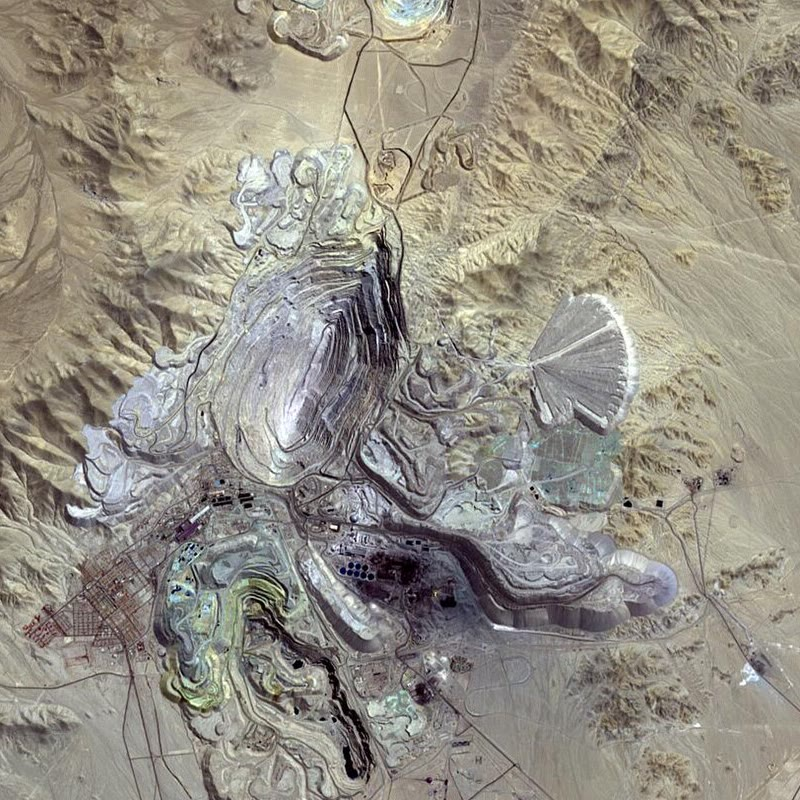
\includegraphics[width=\linewidth]{images/book1/g9-chuquicamata.jpg}
\end{minipage}\hfill
\begin{minipage}[c]{0.5\linewidth}\raggedright
{\small La mine de cuivre de Chuquicamata, dans le \omterm{def:g5:weather-and-climate:desert}{désert} d'Atacama, au
Chili, vue par l'instrument ASTER d'un satellite de la NASA en 2007
(l'image couvre environ \qty{12}{km} de large). La fosse ovale du centre,
exploitée depuis plus d'un siècle, mesure \qty{4.3}{km} de long,
\qty{2.7}{km} de large et \qty{1.1}{km} de profondeur. NASA/METI/AIST/Japan
Space Systems et U.S./Japan ASTER Science Team (domaine public, via
Wikimedia Commons).}
\end{minipage}
% ledger: commons:chuquicamata, earle:chuquicamata
\label{fig:g9:earth-resources:chuquicamata}
\end{omfigure}

\paragraph{Dans les graviers des rivières.} L'or ne rouille pas et ne
s'altère presque pas. Quand l'\omterm{def:g5:water-shapes-the-land:erosion}{érosion} use un filon d'or, l'or est libéré
sous forme de poussière, de paillettes, de grains et parfois de pépites,
et les \omterm{def:g1:landscapes-around-us:water}{rivières} l'emportent vers l'aval. L'or est très dense~: environ
\qty{19}{g/cm^3} pur, contre environ \qty{2.5}{g/cm^3} pour une \omterm{def:g3:stones-pebbles-sand:rock}{roche}
ordinaire. Pendant les \omterm{def:g5:water-shapes-the-land:flood}{crues}, quand tout le lit de \omterm{def:g3:stones-pebbles-sand:sand}{sable} et de \omterm{def:g3:stones-pebbles-sand:pebble}{graviers} se
met en mouvement, les grains d'or, lourds, s'enfoncent peu à peu et se
rassemblent sur la \omterm{def:g3:stones-pebbles-sand:rock}{roche en place}. Les géologues appellent ces \omterm{def:g9:earth-resources:ore-deposit}{gisements}
des \emph{placers}\index{placer}.
% ledger: usgs:gold-placer

\section{Charbon, pétrole et gaz}

Le charbon, le pétrole et le gaz naturel sont les restes d'êtres vivants
enfouis avant d'avoir pu pourrir. Presque toute la matière organique d'une
plante ou d'un animal mort redevient du dioxyde de carbone en quelques
semaines à quelques décennies. Seule la part coupée de l'oxygène de l'air,
au fond d'un marais aux eaux stagnantes ou d'une \omterm{def:g2:water-on-earth:ocean}{mer} profonde, peut être
enfouie et conservée pendant des millions d'années.
% ledger: earle:coal, earle:oil-gas

\begin{omfigure}
\begin{minipage}[c]{0.46\linewidth}\centering
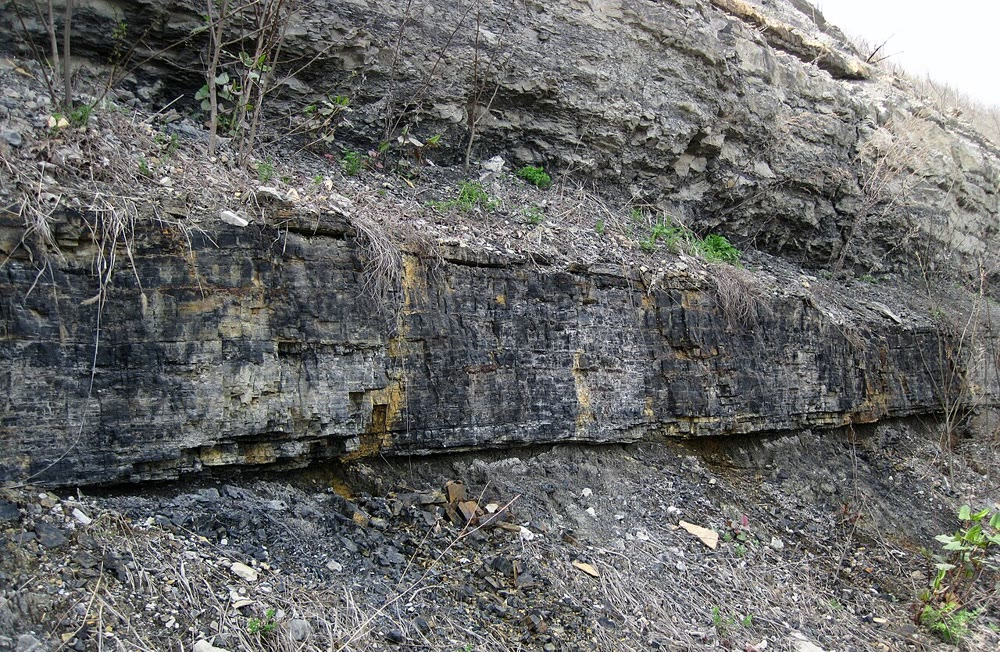
\includegraphics[width=\linewidth]{images/book1/g9-coal-seam.jpg}
\end{minipage}\hfill
\begin{minipage}[c]{0.5\linewidth}\raggedright
{\small Une veine de charbon, la couche sombre qui traverse le milieu,
entre des \omterm{def:g6:rocks-and-minerals:rock-families}{roches sédimentaires}, au bord d'une route de l'Ohio, aux
États-Unis. La veine est horizontale, comme l'était le marais. Photographie
de James St.~John (CC BY 2.0, via Wikimedia Commons).}
\end{minipage}
% ledger: commons:meigs-coal
\label{fig:g9:earth-resources:coal-seam}
\end{omfigure}


\paragraph{Le charbon.} Le charbon naît dans des marais au bord des \omterm{def:g1:landscapes-around-us:water}{rivières}
et des \omterm{def:g5:water-shapes-the-land:delta}{deltas}, sous des \omterm{def:g5:weather-and-climate:climate}{climats} chauds et humides, où les plantes poussent
vite. Les troncs et les feuilles morts tombent dans une eau calme, pauvre
en oxygène, et ne pourrissent pas. Le marais doit durer des siècles, voire
des millénaires, pour former une couche épaisse. Un jour, une \omterm{def:g1:landscapes-around-us:water}{rivière}
change de cours ou déborde, et recouvre le marais de \omterm{def:g3:stones-pebbles-sand:sand}{sable} et de \omterm{def:g3:stones-pebbles-sand:sand}{boue}. À
mesure que les \omterm{def:g7:sediments-and-fossils:sediment}{sédiments} s'accumulent, la couche de plantes est comprimée
et chauffée, et se transforme en charbon~: d'abord un charbon brun et
tendre, contenant environ un tiers de carbone, à quelques centaines de
mètres de profondeur~; puis un charbon noir et dur, contenant jusqu'à
86~\% de carbone, à quelques kilomètres de profondeur. Le charbon extrait
aujourd'hui aux États-Unis, par exemple, a pour l'essentiel de 100 à
300~millions d'années.
% ledger: earle:coal, eia:coal

\begin{omfigure}
\begin{tikzpicture}[x=1cm, y=0.8cm, font=\footnotesize]
  \foreach \i/\t in {0/{(a) un marais boisé~:\\ les plantes mortes\\ s'empilent sous\\ une eau calme},
                     1/{(b) enfouie sous le sable\\ et la boue d'une\\ rivière, la couche\\ est comprimée},
                     2/{(c) plus profond et plus\\ chaud (des centaines\\ de mètres)~: charbon\\ brun et tendre},
                     3/{(d) plus profond encore\\ (des kilomètres)~:\\ charbon noir et dur}} {
    \begin{scope}[xshift=\i*3.35cm]
      \draw[black!40] (0,0) rectangle (2.9,4.2);
      \node[align=center, anchor=north, font=\scriptsize] at (1.45,-0.1) {\t};
    \end{scope}
  }
  % (a) swamp: water, trees, plant layer
  \fill[omSea] (0,2.6) rectangle (2.9,3.1);
  \fill[brown!60!black!70] (0,2.0) rectangle (2.9,2.6);
  \fill[omLithShale] (0,0) rectangle (2.9,2.0);
  \foreach \x in {0.5,1.4,2.3} {
    \draw[brown!50!black, line width=1.2pt] (\x,2.6) -- (\x,3.7);
    \fill[green!45!black] (\x,3.85) circle (0.3);
  }
  % (b) buried
  \begin{scope}[xshift=3.35cm]
    \fill[lith sandstone] (0,2.6) rectangle (2.9,4.0);
    \fill[brown!55!black!80] (0,2.2) rectangle (2.9,2.6);
    \fill[omLithShale] (0,0) rectangle (2.9,2.2);
    \draw[->, thick] (1.45,4.15) -- (1.45,3.45);
  \end{scope}
  % (c) lignite
  \begin{scope}[xshift=6.7cm]
    \fill[lith sandstone] (0,1.9) rectangle (2.9,4.2);
    \fill[brown!45!black] (0,1.65) rectangle (2.9,1.9);
    \fill[omLithShale] (0,0) rectangle (2.9,1.65);
  \end{scope}
  % (d) coal
  \begin{scope}[xshift=10.05cm]
    \fill[lith sandstone] (0,1.25) rectangle (2.9,4.2);
    \fill[black!85] (0,1.1) rectangle (2.9,1.25);
    \fill[omLithShale] (0,0) rectangle (2.9,1.1);
  \end{scope}
\end{tikzpicture}

{\small D'un marais à une veine de charbon (un croquis, sans souci
d'échelle). À mesure que la couche de plantes s'enfonce, elle est
comprimée et chauffée~: l'eau et des gaz la quittent, elle s'amincit, et
sa part de carbone augmente.}
% ledger: earle:coal, eia:coal
\label{fig:g9:earth-resources:coal}
\end{omfigure}


\paragraph{Le pétrole et le gaz.} Le pétrole et la plus grande partie du gaz
naturel proviennent des minuscules plantes et animaux qui vivent dans la
\omterm{def:g2:water-on-earth:ocean}{mer}, comme les diatomées. Leurs restes coulent avec la \omterm{def:g3:stones-pebbles-sand:sand}{boue} jusqu'au fond
de la \omterm{def:g2:water-on-earth:ocean}{mer}, et une partie est enfouie avant de se décomposer. Des millions
d'années et des kilomètres de \omterm{def:g7:sediments-and-fossils:sediment}{sédiments} plus tard, la chaleur et la
pression les transforment~: au-dessous d'environ \qty{2}{km}, entre
environ 60 et \qty{120}{\degreeCelsius}, en pétrole~; plus chaud encore, en
gaz. Le pétrole et le gaz sont plus légers que l'eau. Ils montent
lentement à travers les \omterm{def:g6:water-underground:porosity}{pores} des \omterm{def:g3:stones-pebbles-sand:rock}{roches} \omterm{def:g6:water-underground:permeability}{perméables}, et beaucoup atteignent
la surface et sont perdus. Ceux que nous trouvons ont été arrêtés en
chemin par une couche de \omterm{def:g3:stones-pebbles-sand:rock}{roche} \omterm{def:g6:water-underground:permeability}{imperméable}, souvent au sommet d'un pli en
voûte, où ils s'accumulent~: le gaz en haut, le pétrole au-dessous, et
l'eau en dessous.
% ledger: eia:oil, eia:gas, earle:oil-gas

\begin{omfigure}
\begin{tikzpicture}[x=1cm, y=1cm, font=\footnotesize, >={Stealth[length=2mm]}]
  \def\fold#1{(0,#1) .. controls (3,#1+1.0) and (4.0,#1+1.6) .. (6,#1+1.6) .. controls (8.0,#1+1.6) and (9,#1+1.0) .. (12,#1)}
  % layers from the bottom up
  \fill[omLithShale!60!black!40] (0,0) -- \fold{0.9} -- (12,0) -- cycle;
  \fill[lith sandstone] \fold{0.9} -- (12,2.1) -- (12,2.1) .. controls (9,3.1) and (8.0,3.7) .. (6,3.7) .. controls (4.0,3.7) and (3,3.1) .. (0,2.1) -- cycle;
  \fill[lith shale] (0,2.1) .. controls (3,3.1) and (4.0,3.7) .. (6,3.7) .. controls (8.0,3.7) and (9,3.1) .. (12,2.1) -- (12,3.6) .. controls (9,4.6) and (8.0,5.2) .. (6,5.2) .. controls (4.0,5.2) and (3,4.6) .. (0,3.6) -- cycle;
  \fill[lith sandstone] (0,3.6) .. controls (3,4.6) and (4.0,5.2) .. (6,5.2) .. controls (8.0,5.2) and (9,4.6) .. (12,3.6) -- (12,5.6) -- (0,5.6) -- cycle;
  % gas and oil under the crest of the impermeable layer
  \fill[omWxSun!60] (4.55,3.55) .. controls (5.2,3.69) and (6.8,3.69) .. (7.45,3.55) -- (7.1,3.35) -- (4.9,3.35) -- cycle;
  \fill[black!75] (4.9,3.35) -- (7.1,3.35) -- (8.05,3.05) .. controls (7.0,3.15) and (5.0,3.15) .. (3.95,3.05) -- cycle;
  % arrows: oil creeping up through the permeable layer
  \draw[->, black, thick] (1.4,2.05) -- (2.4,2.55);
  \draw[->, black, thick] (10.6,2.05) -- (9.6,2.55);
  \draw[->, black!70] (3.0,2.65) -- (3.8,2.95);
  \draw[->, black!70] (9.0,2.65) -- (8.2,2.95);
  % labels
  \node[anchor=west, fill=white, fill opacity=0.85, text opacity=1, inner sep=1.5pt] at (0.1,0.45) {boue sombre de l'ancien fond marin~: le pétrole et le gaz s'y forment};
  \node[anchor=east, fill=white, fill opacity=0.85, text opacity=1, inner sep=1.5pt] at (11.9,1.9) {grès perméable};
  \node[anchor=east, fill=white, fill opacity=0.85, text opacity=1, inner sep=1.5pt] at (11.9,3.25) {argilite imperméable};
  \node[anchor=south, fill=white, fill opacity=0.85, text opacity=1, inner sep=1.5pt] at (6,5.25) {roches de surface};
  \node[font=\scriptsize] at (6,3.48) {gaz};
  \node[font=\scriptsize, text=white] at (6,3.22) {pétrole};
\end{tikzpicture}

{\small Pétrole et gaz arrêtés sous une couche \omterm{def:g6:water-underground:permeability}{imperméable} au sommet d'un
pli en voûte (un croquis, sans souci d'échelle~; l'eau qui remplit le reste
du grès n'est pas représentée). Sous le pli, ils montent à travers le grès
\omterm{def:g6:water-underground:permeability}{perméable} (flèches) et s'accumulent sous la crête~: le gaz en haut, le
pétrole au-dessous.}
% ledger: earle:oil-gas
\label{fig:g9:earth-resources:oil}
\end{omfigure}

\section{L'eau du sous-sol}

L'\omterm{def:g6:water-underground:groundwater}{eau souterraine} est elle aussi une ressource de la Terre, celle que nous
utilisons chaque jour. Contrairement à un métal ou au charbon, elle se
renouvelle~: la \omterm{def:g4:clouds-rain-snow:precipitation}{pluie} recharge les \omterm{def:g6:water-underground:aquifer}{aquifères}. Mais elle se renouvelle
lentement, et seulement au rythme où la \omterm{def:g4:clouds-rain-snow:precipitation}{pluie} s'infiltre. Un \omterm{def:g6:water-underground:aquifer}{aquifère}
pompé plus vite qu'il ne se recharge voit sa nappe baisser, et les \omterm{def:g6:water-underground:spring}{puits}
s'assèchent (\cref{ch:g6:water-underground}). L'\omterm{def:g6:water-underground:groundwater}{eau souterraine} n'est une
ressource renouvelable que tant qu'on ne la prélève pas plus vite qu'elle
ne se renouvelle.
% ledger: wss:aquifer

\section{Le sable et le gravier}

Le matériau solide que l'on extrait du sol en plus grande quantité n'est
ni le charbon ni un minerai métallique~: c'est le \omterm{def:g3:stones-pebbles-sand:sand}{sable} et le gravier.
% ledger: tos:sand

\begin{definition}[Granulats]\label{def:g9:earth-resources:aggregate}
Les \emph{granulats}\index{granulats} sont le \omterm{def:g3:stones-pebbles-sand:sand}{sable}, le gravier et la
pierre concassée utilisés dans la construction~: dans le béton, sous les
routes et les voies ferrées, et pour remblayer le sol.
\end{definition}
% ledger: usgs:aggregate, tos:sand

La plus grande partie du \omterm{def:g3:stones-pebbles-sand:sand}{sable} sert à faire du béton, un mélange de \omterm{def:g3:stones-pebbles-sand:sand}{sable},
de gravier, d'eau et de ciment. En 2019, le monde avait besoin d'environ
50~milliards de tonnes de \omterm{def:g3:stones-pebbles-sand:sand}{sable} et de gravier par an,
soit $5 \times 10^{10}$ tonnes, ou environ \qty{18}{kg} par habitant de la
Terre et par jour. Le \omterm{def:g3:stones-pebbles-sand:sand}{sable} et le gravier sont extraits de carrières à
terre, du lit des \omterm{def:g1:landscapes-around-us:water}{rivières} et, de plus en plus, du fond de la \omterm{def:g2:water-on-earth:ocean}{mer}. Prélevés
dans une \omterm{def:g1:landscapes-around-us:water}{rivière}, ils laissent moins de \omterm{def:g3:stones-pebbles-sand:sand}{sable} atteindre la \omterm{def:g1:landscapes-around-us:water}{côte}, et les
plages situées en aval reculent.
% ledger: tos:sand

\begin{omfigure}
\begin{minipage}[c]{0.46\linewidth}\centering
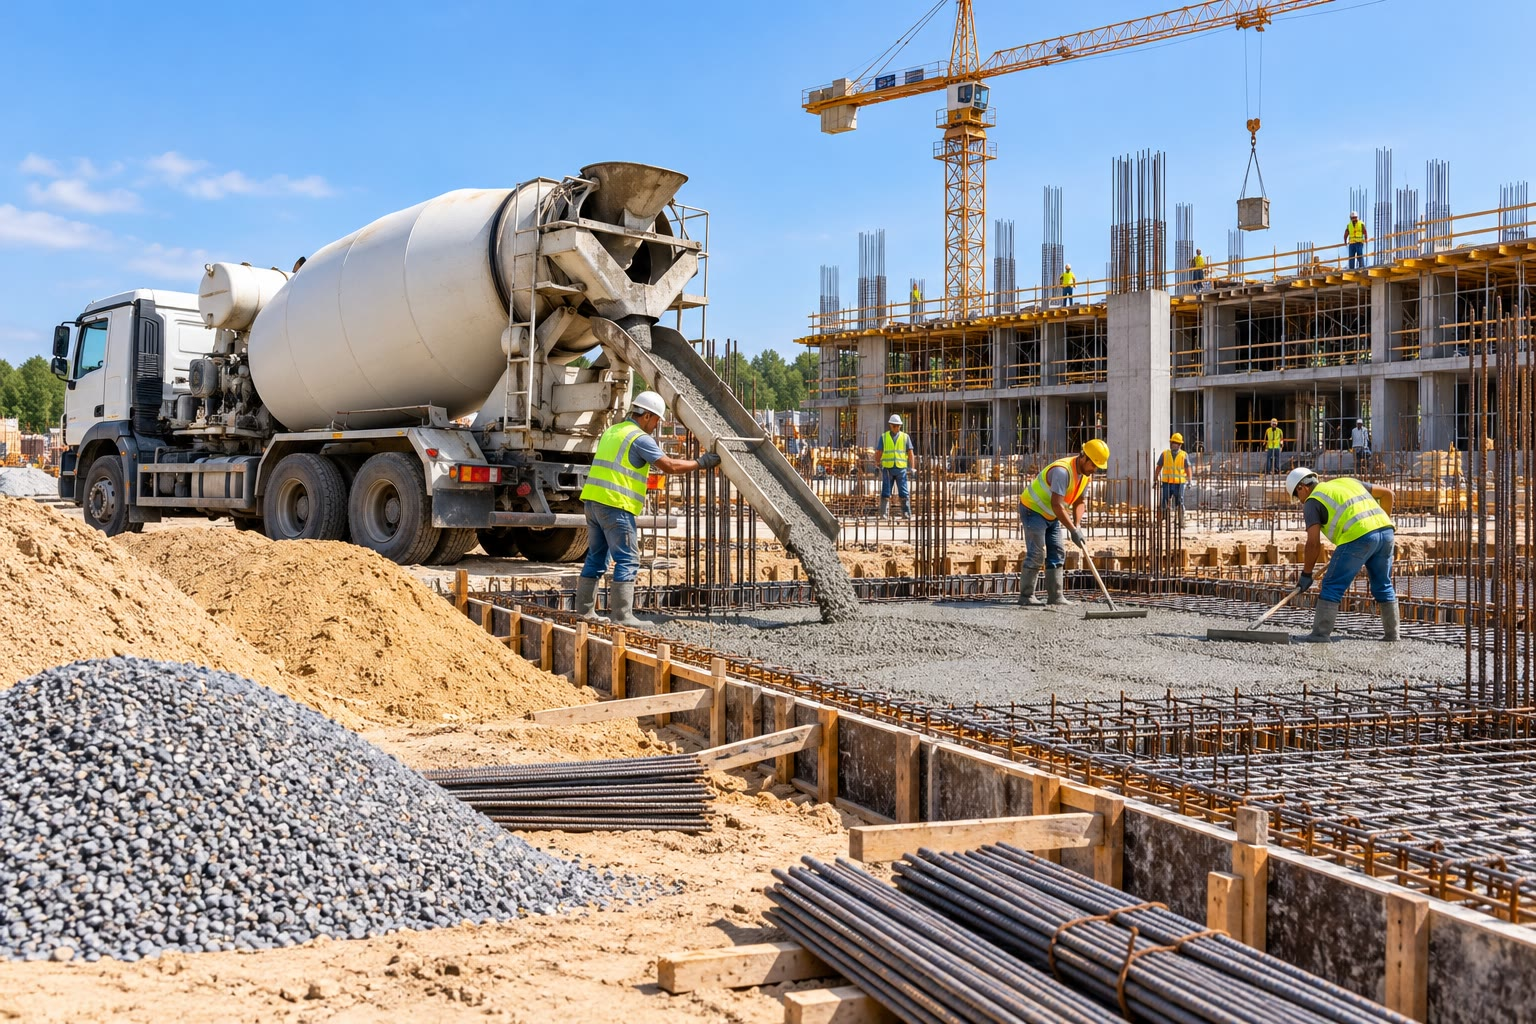
\includegraphics[width=\linewidth]{images/book1/ai/g9-building-site.jpg}
\end{minipage}\hfill
\begin{minipage}[c]{0.5\linewidth}\raggedright
{\small Les \omterm{def:g9:earth-resources:aggregate}{granulats} au travail~: des tas de \omterm{def:g3:stones-pebbles-sand:sand}{sable} et de gravier à côté
d'un camion toupie qui coule la dalle d'un nouveau bâtiment (illustration
générée par IA d'une scène générique).}
\end{minipage}
\label{fig:g9:earth-resources:building-site}
\end{omfigure}

\section{Renouvelable ou épuisable~?}

Une ressource que la nature renouvelle en moins d'une vie humaine, comme
l'eau d'un \omterm{def:g6:water-underground:aquifer}{aquifère} qui n'est pas surexploité, peut être utilisée
indéfiniment. Un \omterm{def:g9:earth-resources:ore-deposit}{gisement} de minerai, une veine de charbon ou un gisement
de pétrole ont mis des millions d'années à se former. Nous les utilisons
en quelques décennies~: à notre échelle de temps, ils ne se renouvellent
pas du tout.
% ledger: eia:coal, earle:coal

\begin{omfigure}
\begin{tikzpicture}
\begin{axis}[xmode=log, width=12.5cm, height=4.6cm, xmin=10, xmax=1e9, ymin=0.4, ymax=4.6,
  ytick=\empty, xlabel={années (échelle logarithmique)}, label style={font=\small},
  xtick={10,100,1000,1e4,1e5,1e6,1e7,1e8,1e9},
  xticklabels={$10$,$10^2$,$10^3$,$10^4$,$10^5$,$10^6$,$10^7$,$10^8$,$10^9$},
  tick label style={font=\footnotesize}, xmajorgrids, grid style={black!12}, clip=false]
\addplot[only marks, mark=|, mark size=4pt, line width=4pt, omWarm,
  error bars/.cd, x dir=plus, x explicit, error bar style={line width=4pt, omWarm}, error mark=none]
  table[x=lo_yr, y=y, x error expr=\thisrow{hi_yr}-\thisrow{lo_yr}] {figdata/out/grade-9-concentration-times.dat};
\node[anchor=west, font=\footnotesize, fill=white, inner sep=1pt] at (axis cs:1500,4) {un marais forme une épaisse couche de plantes};
\node[anchor=east, font=\footnotesize, fill=white, inner sep=1pt] at (axis cs:6e7,3) {âge du charbon extrait aux États-Unis};
\node[anchor=west, font=\footnotesize, fill=white, inner sep=1pt] at (axis cs:150,2) {Chuquicamata, exploitée à ce jour (plus d'un siècle)};
\node[anchor=west, font=\footnotesize, fill=white, inner sep=1pt] at (axis cs:65,1) {réserves mondiales de cuivre, au rythme de 2024};
\end{axis}
\end{tikzpicture}

{\small Temps de formation et temps d'utilisation, sur une échelle où
chaque graduation vaut dix fois la précédente. Le charbon est environ un
million de fois plus ancien que le temps qu'une mine met à vider un
\omterm{def:g9:earth-resources:ore-deposit}{gisement}.}
% ledger: earle:coal, eia:coal, earle:chuquicamata, usgs:mcs-copper (figdata/grade-9/concentration.py, part times)
\label{fig:g9:earth-resources:times}
\end{omfigure}

Combien de temps une ressource durera-t-elle~? Les géologues ne comptent
que ce qui est connu et peut être extrait.

\begin{definition}[Réserves]\label{def:g9:earth-resources:reserve}
Les \emph{réserves}\index{reserves@réserves} d'une ressource minérale sont la part des
\omterm{def:g9:earth-resources:ore-deposit}{gisements} connus qui peut être extraite avec profit, avec les techniques et
les prix du moment.
\end{definition}
% ledger: usgs:mcs-reserves

Les \omterm{def:g9:earth-resources:reserve}{réserves} ne sont pas tout ce qui se trouve dans le sol. Elles
augmentent quand on découvre de nouveaux \omterm{def:g9:earth-resources:ore-deposit}{gisements}, quand les techniques
progressent ou quand les prix montent, et elles diminuent à mesure que les
\omterm{def:g9:earth-resources:ore-deposit}{gisements} sont exploités. En 1970, les \omterm{def:g9:earth-resources:reserve}{réserves} mondiales de cuivre étaient
estimées à 280~millions de tonnes. Depuis, environ 700~millions de tonnes
de cuivre ont été extraites, deux fois et demie ces \omterm{def:g9:earth-resources:reserve}{réserves}, et pourtant
les \omterm{def:g9:earth-resources:reserve}{réserves} de 2024 étaient estimées à 980~millions de tonnes.
% ledger: usgs:mcs-reserves

\begin{dated}{2025}
En 2024, les mines du monde ont produit environ 23~millions de tonnes de
cuivre. À ce rythme, les \omterm{def:g9:earth-resources:reserve}{réserves} de 980~millions de tonnes dureraient $980 \div 23
\approx 43$ ans. Un tel nombre n'est pas la date à laquelle le cuivre
s'épuisera~: c'est une mesure du cuivre connu et qu'il vaut la peine
d'extraire aujourd'hui.
\end{dated}
% ledger: usgs:mcs-copper (figdata/grade-9/concentration.py: 42.6 years)

Un métal, contrairement au charbon ou au pétrole, n'est pas détruit quand
on l'utilise~: le recyclage des matériaux, vu dans les livres de chimie,
le rend de nouveau disponible. Le cuivre d'un vieux câble, d'un moteur mis
à la ferraille ou des chutes d'une usine peut être refondu et affiné de
nouveau. Aux États-Unis, en 2024, le cuivre récupéré à partir de déchets
représentait environ \qty{35}{\%} de tout le cuivre utilisé.
% ledger: usgs:mcs-copper-scrap

\begin{omfigure}
\begin{tikzpicture}[font=\footnotesize, node distance=1.2cm,
  box/.style={draw=black!60, fill=black!4, rounded corners=2pt, align=center, minimum height=0.9cm, inner sep=3pt},
  flow/.style={-{Stealth[length=2.2mm]}, line width=0.9pt, black!70}]
  \node[box, fill=omWarm!12] (ore) at (0,0) {gisement\\(roche à \qty{0.5}{\%}\\de cuivre)};
  \node[box] (metal) at (4.2,0) {cuivre métal};
  \node[box] (things) at (8.2,0) {câbles, tuyaux,\\moteurs};
  \node[box, fill=blue!8] (scrap) at (6.2,-2.1) {déchets};
  \node[box, fill=black!12] (waste) at (0,-2.1) {roche broyée\\restante};
  \draw[flow] (ore) -- node[above, align=center] {extraire,\\ broyer,} node[below] {concentrer} (metal);
  \draw[flow] (metal) -- node[above] {fabriquer} (things);
  \draw[flow] (things) |- node[pos=0.25, right] {jetés} (scrap);
  \draw[flow] (scrap) -| node[pos=0.75, left] {refondre, affiner} (metal);
  \draw[flow] (ore) -- (waste);
\end{tikzpicture}

{\small Deux chemins vers le cuivre métal~: depuis un minerai, à travers
des tonnes de \omterm{def:g3:stones-pebbles-sand:rock}{roche} extraite et broyée, ou depuis les déchets, refondus et
affinés de nouveau.}
\end{omfigure}

\begin{example}[La roche qu'épargne le recyclage]\label{ex:g9:earth-resources:recycling}
Un minerai à \qty{0.5}{\%} de cuivre contient \qty{5}{kg} de cuivre par
tonne de \omterm{def:g3:stones-pebbles-sand:rock}{roche}. Pour produire une tonne de cuivre, il faut extraire,
broyer et traiter environ $1000 \div 5 = 200$ tonnes de minerai, et
presque tout finit en stériles. Chaque tonne de cuivre produite à partir de
déchets laisse ces 200 tonnes de \omterm{def:g3:stones-pebbles-sand:rock}{roche} dans le sol --- et le \omterm{def:g9:earth-resources:ore-deposit}{gisement} dure
plus longtemps.
% ledger: perkins:ore-grades (computed)
\end{example}


\section{Exercices}

\begin{exercise}[$\star$]\label{exo:g9:earth-resources:1}
Complète avec le mot qui convient (\omterm{def:g9:earth-resources:ore-deposit}{gisement}, \omterm{def:g9:earth-resources:ore-deposit}{facteur de concentration},
\omterm{def:g9:earth-resources:aggregate}{granulats}, \omterm{def:g9:earth-resources:reserve}{réserves}). (a) Le \omterm{def:g3:stones-pebbles-sand:sand}{sable} utilisé dans le béton fait partie des
\ldots\ (b) La part du cuivre connu qui peut être extraite avec profit
aujourd'hui forme les \ldots\ de cuivre. (c) Une \omterm{def:g3:stones-pebbles-sand:rock}{roche} où un métal est
assez riche pour être exploité est un \ldots\ (d) Le nombre de fois qu'un
métal a été concentré est son \ldots
\end{exercise}

\begin{exercise}[$\star$]\label{exo:g9:earth-resources:2}
% ledger: earle:magmatic, usgs:gold-lode, usgs:gold-placer
Quelle façon de concentrer un métal chaque phrase décrit-elle~: dans le
\omterm{def:g7:volcanoes:magma}{magma}, dans les fissures par l'eau chaude, ou dans les \omterm{def:g3:stones-pebbles-sand:pebble}{graviers} des
\omterm{def:g1:landscapes-around-us:water}{rivières}~? (a) Des pépites d'or reposent sur la \omterm{def:g3:stones-pebbles-sand:rock}{roche en place}, sous les
\omterm{def:g3:stones-pebbles-sand:pebble}{graviers} d'un ruisseau. (b) De l'eau chaude remplit une fissure de quartz
et d'or. (c) Une couche de \omterm{def:g6:rocks-and-minerals:mineral}{minéraux} lourds de nickel se trouve au fond
d'un ancien corps de \omterm{def:g7:volcanoes:magma}{magma}. (d) L'or est libéré d'un filon par l'\omterm{def:g5:water-shapes-the-land:erosion}{érosion}.
\end{exercise}

\begin{exercise}[$\star$]\label{exo:g9:earth-resources:3}
% ledger: earle:coal, eia:coal
Remets ces étapes dans l'ordre~: (a) la couche de plantes est enfouie sous
le \omterm{def:g3:stones-pebbles-sand:sand}{sable} d'une \omterm{def:g1:landscapes-around-us:water}{rivière}~; (b) des arbres poussent dans un marais~; (c) un
charbon noir et dur se forme à des kilomètres de profondeur~; (d) des
plantes mortes s'empilent sous une eau calme~; (e) un charbon brun et
tendre se forme.
\end{exercise}

\begin{exercise}[$\star$]\label{exo:g9:earth-resources:4}
À l'échelle d'une vie humaine, chaque ressource est-elle renouvelable ou
non~? Explique en une phrase. (a) Le charbon. (b) L'eau d'un \omterm{def:g6:water-underground:aquifer}{aquifère}
pompé moins que la \omterm{def:g4:clouds-rain-snow:precipitation}{pluie} ne le recharge. (c) Le minerai de cuivre. (d) Le
même \omterm{def:g6:water-underground:aquifer}{aquifère} pompé deux fois plus vite qu'il ne se recharge.
\end{exercise}

\begin{exercise}[$\star\star$]\label{exo:g9:earth-resources:5}
% ledger: perkins:ore-grades
Calcule le \omterm{def:g9:earth-resources:ore-deposit}{facteur de concentration}, puis écris-le sous forme de puissance
de dix, arrondie~: (a) le zinc, \qty{0.007}{\%} dans la \omterm{def:g6:inside-the-earth:layers}{croûte}, minerai à
partir de \qty{4}{\%}~; (b) l'étain, \qty{0.0002}{\%} dans la \omterm{def:g6:inside-the-earth:layers}{croûte},
minerai à partir de \qty{0.5}{\%}~; (c) le fer, \qty{5.6}{\%} dans la
\omterm{def:g6:inside-the-earth:layers}{croûte}, minerai à partir de \qty{20}{\%}. (d) Pourquoi le fer a-t-il
besoin de si peu de concentration~?
\end{exercise}

\begin{exercise}[$\star\star$]\label{exo:g9:earth-resources:6}
% ledger: usgs:gold-placer
L'or pur a une masse volumique d'environ \qty{19.3}{g/cm^3}~; une \omterm{def:g3:stones-pebbles-sand:rock}{roche}
ordinaire, d'environ \qty{2.5}{g/cm^3}. (a) Combien de fois l'or est-il
plus dense~? (b) Quelle est la masse d'un grain d'or de \qty{0.01}{cm^3},
et celle d'un grain de \omterm{def:g3:stones-pebbles-sand:rock}{roche} de même taille~? (c) Explique pourquoi,
pendant une \omterm{def:g5:water-shapes-the-land:flood}{crue}, l'or finit au fond des \omterm{def:g3:stones-pebbles-sand:pebble}{graviers}, sur la \omterm{def:g3:stones-pebbles-sand:rock}{roche en place}.
\end{exercise}

\begin{exercise}[$\star\star$]\label{exo:g9:earth-resources:7}
% ledger: perkins:ore-grades, earle:ore-grades (figdata/grade-9/concentration.py)
Utilise le graphique des \omterm{def:g9:earth-resources:ore-deposit}{facteurs de concentration}. (a) Quels métaux ont
besoin d'un facteur supérieur à $10^3$~? (b) Entre quelles puissances de
dix se situe le cuivre~? (c) Combien de fois plus le chrome doit-il être
concentré que l'aluminium~? (d) Lequel des sept métaux t'attends-tu à voir
exploité dans le plus petit nombre d'endroits~? Explique.
\end{exercise}

\begin{exercise}[$\star\star$]\label{exo:g9:earth-resources:8}
% ledger: tos:sand
Le monde a besoin d'environ \qty{18}{kg} de \omterm{def:g3:stones-pebbles-sand:sand}{sable} et de gravier par
habitant et par jour. (a) Combien cela fait-il par habitant en un an, en
tonnes~? (b) Écris 50 milliards de tonnes en notation scientifique. (c) Un
camion transporte \qty{25}{t}. Combien de jours faut-il pour que la part
d'une personne le remplisse~? (d) Pourquoi prélever du \omterm{def:g3:stones-pebbles-sand:sand}{sable} dans une
\omterm{def:g1:landscapes-around-us:water}{rivière} peut-il faire reculer une plage située en aval~?
\end{exercise}

\begin{exercise}[$\star\star$]\label{exo:g9:earth-resources:9}
% ledger: earle:oil-gas, eia:oil
(a) De quels êtres vivants proviennent la plus grande partie du pétrole et
du gaz~? (b) Au-dessous d'environ \qty{2}{km}, à quelles températures le
pétrole se forme-t-il~? (c) Pourquoi le pétrole et le gaz montent-ils à
travers les \omterm{def:g3:stones-pebbles-sand:rock}{roches}~? (d) Quel type de \omterm{def:g3:stones-pebbles-sand:rock}{roche} les arrête, et où
s'accumulent-ils~?
\end{exercise}

\begin{exercise}[$\star\star$]\label{exo:g9:earth-resources:10}
% ledger: earle:chuquicamata
La mine de Chuquicamata a produit plus de 29~millions de tonnes de cuivre
en plus de 100 ans. (a) Écris 29~millions de tonnes en notation
scientifique. (b) Quelle est, en gros, la production moyenne par an~?
(c) Si le minerai contenait \qty{1}{\%} de cuivre, combien de tonnes de
minerai a-t-il fallu extraire pour obtenir 29~millions de tonnes de
cuivre~? Utilise la notation scientifique. (d) Pourquoi une mine d'un
minerai aussi pauvre doit-elle être si grande~?
\end{exercise}

\begin{exercise}[$\star\star\star$]\label{exo:g9:earth-resources:11}
% ledger: usgs:mcs-reserves, usgs:mcs-copper
En 1970, les \omterm{def:g9:earth-resources:reserve}{réserves} mondiales de cuivre étaient estimées à 280~millions
de tonnes. De 1970 à 2024, environ 697~millions de tonnes ont été extraites,
et les \omterm{def:g9:earth-resources:reserve}{réserves} de 2024 étaient de 980~millions de tonnes, avec
23~millions de tonnes extraites en 2024. (a) Si les \omterm{def:g9:earth-resources:reserve}{réserves} de 1970
avaient représenté tout le cuivre existant, quand se seraient-elles
épuisées~? Compare avec ce qui a été extrait. (b) Combien de fois les
\omterm{def:g9:earth-resources:reserve}{réserves} de 2024 sont-elles plus grandes que celles de 1970~? (c) Calcule
combien d'années les \omterm{def:g9:earth-resources:reserve}{réserves} de 2024 dureraient au rythme de 2024.
(d) Donne deux raisons pour lesquelles des \omterm{def:g9:earth-resources:reserve}{réserves} peuvent augmenter alors
même qu'on les exploite.
\end{exercise}

\begin{exercise}[$\star\star\star$]\label{exo:g9:earth-resources:12}
% ledger: earle:coal, eia:coal
Une veine de charbon a $3 \times 10^8$ ans. Son marais a duré $2 \times 10^3$
ans, et la veine est épuisée en 50 ans. (a) Écris 50 ans en notation
scientifique. (b) Combien de fois plus longtemps que l'exploitation le
marais a-t-il duré~? (c) Combien de fois la veine est-elle plus ancienne
que la durée de l'exploitation~? (d) Utilise ces nombres pour expliquer
pourquoi le charbon est dit ressource non renouvelable.
\end{exercise}

\section{Problème~: du béton pour une ville nouvelle}

\begin{problem}[{Problème du week-end --- une ville nouvelle est construite
avec le sable d'une carrière voisine~; la réponse finale est le nombre
d'années que dureraient les réserves de sable de la carrière}]
\label{pb:g9:earth-resources:1}
% ledger: usgs:aggregate (about 100 and 300 t per home), tos:sand (figdata/grade-9/concentration.py, part problem: exercise data)
Une ville nouvelle de \num{2000} logements doit être construite en dix ans,
près d'une ancienne sablière creusée dans les \omterm{def:g3:stones-pebbles-sand:pebble}{graviers} d'une terrasse
alluviale. En comptant sa part des rues, des écoles et des commerces,
chaque logement demande environ \qty{300}{t} de \omterm{def:g9:earth-resources:aggregate}{granulats}, dont
\qty{40}{\%} de \omterm{def:g3:stones-pebbles-sand:sand}{sable}. La couche de \omterm{def:g3:stones-pebbles-sand:sand}{sable} de la carrière mesure
\qty{1.2}{km} de long, \qty{500}{m} de large et \qty{5}{m} d'épaisseur~;
un mètre cube de son \omterm{def:g3:stones-pebbles-sand:sand}{sable} a une masse de \qty{1.6}{t}. La carrière vend
aussi \num{136000} tonnes de \omterm{def:g3:stones-pebbles-sand:sand}{sable} par an au reste de la région.

\noindent\textbf{Partie I --- Combien de sable~?}\par\nopagebreak
\begin{enumerate}[beginpenalty=10000]
  \item Une maison familiale seule demande environ \qty{100}{t} de
        \omterm{def:g9:earth-resources:aggregate}{granulats}. Écris cette masse en kilogrammes, en notation
        scientifique.
  \item Combien de tonnes de \omterm{def:g9:earth-resources:aggregate}{granulats} la ville entière demandera-t-elle~?
  \item Combien de tonnes cela fait-il par an, sur les dix ans~?
  \item Combien de tonnes de \omterm{def:g3:stones-pebbles-sand:sand}{sable} par an la ville demande-t-elle~?
\end{enumerate}

\noindent\textbf{Partie II --- Les réserves.}\par\nopagebreak
\begin{enumerate}[resume, beginpenalty=10000]
  \item Calcule le volume de la couche de \omterm{def:g3:stones-pebbles-sand:sand}{sable}, en mètres cubes, en
        notation scientifique.
  \item Un tiers de la couche se trouve sous un village et une route et ne
        sera pas creusé. Quel volume peut être extrait~?
  \item Quelle est la masse de ces \omterm{def:g9:earth-resources:reserve}{réserves}, en tonnes~?
  \item Combien de tonnes de \omterm{def:g3:stones-pebbles-sand:sand}{sable} la carrière vendra-t-elle chaque année,
        à la ville et à la région réunies~?
\end{enumerate}

\noindent\textbf{Partie III --- Renouvelable ou non~?}\par\nopagebreak
\begin{enumerate}[resume, beginpenalty=10000]
  \item Chaque année, la \omterm{def:g1:landscapes-around-us:water}{rivière} apporte environ \num{2000} tonnes de \omterm{def:g3:stones-pebbles-sand:sand}{sable}
        neuf dans le secteur. Combien de fois plus de \omterm{def:g3:stones-pebbles-sand:sand}{sable} la carrière
        vend-elle~?
  \item À l'échelle de la vie de la ville, ce \omterm{def:g3:stones-pebbles-sand:sand}{sable} est-il une ressource
        renouvelable~? Explique.
  \item Si la ville remplaçait un quart de son \omterm{def:g3:stones-pebbles-sand:sand}{sable} par du vieux béton
        concassé, combien de tonnes de \omterm{def:g3:stones-pebbles-sand:sand}{sable} économiserait-elle chaque
        année~?
  \item Sans ce recyclage, combien d'années les \omterm{def:g9:earth-resources:reserve}{réserves} de \omterm{def:g3:stones-pebbles-sand:sand}{sable} de la
        carrière dureraient-elles~?
\end{enumerate}
\end{problem}
